% Created by tikzDevice version 0.12.3.1 on 2021-04-04 17:56:42
% !TEX encoding = UTF-8 Unicode
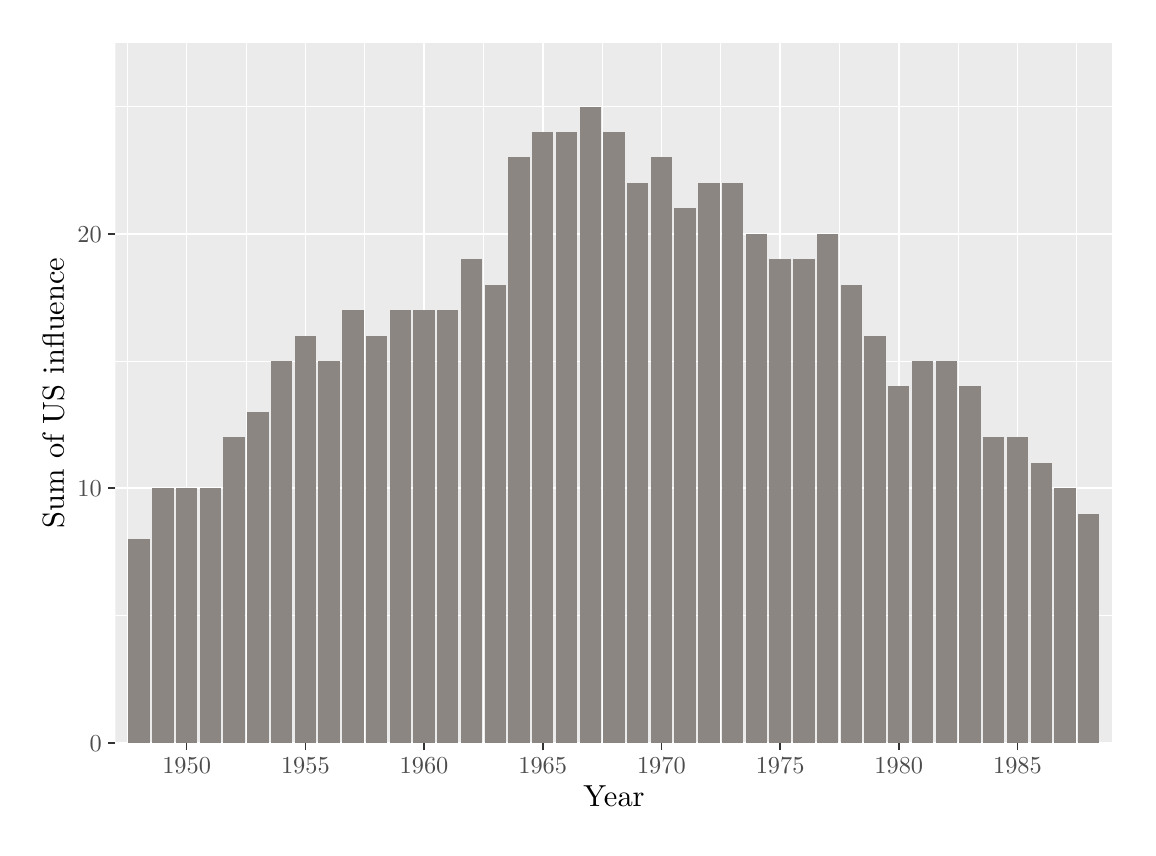
\begin{tikzpicture}[x=1pt,y=1pt]
\definecolor{fillColor}{RGB}{255,255,255}
\path[use as bounding box,fill=fillColor,fill opacity=0.00] (0,0) rectangle (397.48,289.08);
\begin{scope}
\path[clip] (  0.00,  0.00) rectangle (397.48,289.08);
\definecolor{drawColor}{RGB}{255,255,255}
\definecolor{fillColor}{RGB}{255,255,255}

\path[draw=drawColor,line width= 0.6pt,line join=round,line cap=round,fill=fillColor] (  0.00,  0.00) rectangle (397.48,289.08);
\end{scope}
\begin{scope}
\path[clip] ( 31.71, 30.69) rectangle (391.98,283.58);
\definecolor{fillColor}{gray}{0.92}

\path[fill=fillColor] ( 31.71, 30.69) rectangle (391.98,283.58);
\definecolor{drawColor}{RGB}{255,255,255}

\path[draw=drawColor,line width= 0.3pt,line join=round] ( 31.71, 76.67) --
	(391.98, 76.67);

\path[draw=drawColor,line width= 0.3pt,line join=round] ( 31.71,168.63) --
	(391.98,168.63);

\path[draw=drawColor,line width= 0.3pt,line join=round] ( 31.71,260.59) --
	(391.98,260.59);

\path[draw=drawColor,line width= 0.3pt,line join=round] ( 36.00, 30.69) --
	( 36.00,283.58);

\path[draw=drawColor,line width= 0.3pt,line join=round] ( 78.89, 30.69) --
	( 78.89,283.58);

\path[draw=drawColor,line width= 0.3pt,line join=round] (121.78, 30.69) --
	(121.78,283.58);

\path[draw=drawColor,line width= 0.3pt,line join=round] (164.67, 30.69) --
	(164.67,283.58);

\path[draw=drawColor,line width= 0.3pt,line join=round] (207.56, 30.69) --
	(207.56,283.58);

\path[draw=drawColor,line width= 0.3pt,line join=round] (250.45, 30.69) --
	(250.45,283.58);

\path[draw=drawColor,line width= 0.3pt,line join=round] (293.34, 30.69) --
	(293.34,283.58);

\path[draw=drawColor,line width= 0.3pt,line join=round] (336.23, 30.69) --
	(336.23,283.58);

\path[draw=drawColor,line width= 0.3pt,line join=round] (379.12, 30.69) --
	(379.12,283.58);

\path[draw=drawColor,line width= 0.6pt,line join=round] ( 31.71, 30.69) --
	(391.98, 30.69);

\path[draw=drawColor,line width= 0.6pt,line join=round] ( 31.71,122.65) --
	(391.98,122.65);

\path[draw=drawColor,line width= 0.6pt,line join=round] ( 31.71,214.61) --
	(391.98,214.61);

\path[draw=drawColor,line width= 0.6pt,line join=round] ( 57.45, 30.69) --
	( 57.45,283.58);

\path[draw=drawColor,line width= 0.6pt,line join=round] (100.34, 30.69) --
	(100.34,283.58);

\path[draw=drawColor,line width= 0.6pt,line join=round] (143.23, 30.69) --
	(143.23,283.58);

\path[draw=drawColor,line width= 0.6pt,line join=round] (186.11, 30.69) --
	(186.11,283.58);

\path[draw=drawColor,line width= 0.6pt,line join=round] (229.00, 30.69) --
	(229.00,283.58);

\path[draw=drawColor,line width= 0.6pt,line join=round] (271.89, 30.69) --
	(271.89,283.58);

\path[draw=drawColor,line width= 0.6pt,line join=round] (314.78, 30.69) --
	(314.78,283.58);

\path[draw=drawColor,line width= 0.6pt,line join=round] (357.67, 30.69) --
	(357.67,283.58);
\definecolor{fillColor}{RGB}{139,134,130}

\path[fill=fillColor] ( 36.43, 30.69) rectangle ( 44.15,104.26);

\path[fill=fillColor] ( 45.01, 30.69) rectangle ( 52.73,122.65);

\path[fill=fillColor] ( 53.59, 30.69) rectangle ( 61.31,122.65);

\path[fill=fillColor] ( 62.16, 30.69) rectangle ( 69.88,122.65);

\path[fill=fillColor] ( 70.74, 30.69) rectangle ( 78.46,141.04);

\path[fill=fillColor] ( 79.32, 30.69) rectangle ( 87.04,150.24);

\path[fill=fillColor] ( 87.90, 30.69) rectangle ( 95.62,168.63);

\path[fill=fillColor] ( 96.48, 30.69) rectangle (104.20,177.82);

\path[fill=fillColor] (105.05, 30.69) rectangle (112.77,168.63);

\path[fill=fillColor] (113.63, 30.69) rectangle (121.35,187.02);

\path[fill=fillColor] (122.21, 30.69) rectangle (129.93,177.82);

\path[fill=fillColor] (130.79, 30.69) rectangle (138.51,187.02);

\path[fill=fillColor] (139.37, 30.69) rectangle (147.09,187.02);

\path[fill=fillColor] (147.94, 30.69) rectangle (155.66,187.02);

\path[fill=fillColor] (156.52, 30.69) rectangle (164.24,205.41);

\path[fill=fillColor] (165.10, 30.69) rectangle (172.82,196.22);

\path[fill=fillColor] (173.68, 30.69) rectangle (181.40,242.20);

\path[fill=fillColor] (182.25, 30.69) rectangle (189.97,251.39);

\path[fill=fillColor] (190.83, 30.69) rectangle (198.55,251.39);

\path[fill=fillColor] (199.41, 30.69) rectangle (207.13,260.59);

\path[fill=fillColor] (207.99, 30.69) rectangle (215.71,251.39);

\path[fill=fillColor] (216.57, 30.69) rectangle (224.29,233.00);

\path[fill=fillColor] (225.14, 30.69) rectangle (232.86,242.20);

\path[fill=fillColor] (233.72, 30.69) rectangle (241.44,223.81);

\path[fill=fillColor] (242.30, 30.69) rectangle (250.02,233.00);

\path[fill=fillColor] (250.88, 30.69) rectangle (258.60,233.00);

\path[fill=fillColor] (259.46, 30.69) rectangle (267.18,214.61);

\path[fill=fillColor] (268.03, 30.69) rectangle (275.75,205.41);

\path[fill=fillColor] (276.61, 30.69) rectangle (284.33,205.41);

\path[fill=fillColor] (285.19, 30.69) rectangle (292.91,214.61);

\path[fill=fillColor] (293.77, 30.69) rectangle (301.49,196.22);

\path[fill=fillColor] (302.35, 30.69) rectangle (310.07,177.82);

\path[fill=fillColor] (310.92, 30.69) rectangle (318.64,159.43);

\path[fill=fillColor] (319.50, 30.69) rectangle (327.22,168.63);

\path[fill=fillColor] (328.08, 30.69) rectangle (335.80,168.63);

\path[fill=fillColor] (336.66, 30.69) rectangle (344.38,159.43);

\path[fill=fillColor] (345.24, 30.69) rectangle (352.96,141.04);

\path[fill=fillColor] (353.81, 30.69) rectangle (361.53,141.04);

\path[fill=fillColor] (362.39, 30.69) rectangle (370.11,131.84);

\path[fill=fillColor] (370.97, 30.69) rectangle (378.69,122.65);

\path[fill=fillColor] (379.55, 30.69) rectangle (387.27,113.45);
\end{scope}
\begin{scope}
\path[clip] (  0.00,  0.00) rectangle (397.48,289.08);
\definecolor{drawColor}{gray}{0.30}

\node[text=drawColor,anchor=base east,inner sep=0pt, outer sep=0pt, scale=  0.88] at ( 26.76, 27.66) {0};

\node[text=drawColor,anchor=base east,inner sep=0pt, outer sep=0pt, scale=  0.88] at ( 26.76,119.62) {10};

\node[text=drawColor,anchor=base east,inner sep=0pt, outer sep=0pt, scale=  0.88] at ( 26.76,211.58) {20};
\end{scope}
\begin{scope}
\path[clip] (  0.00,  0.00) rectangle (397.48,289.08);
\definecolor{drawColor}{gray}{0.20}

\path[draw=drawColor,line width= 0.6pt,line join=round] ( 28.96, 30.69) --
	( 31.71, 30.69);

\path[draw=drawColor,line width= 0.6pt,line join=round] ( 28.96,122.65) --
	( 31.71,122.65);

\path[draw=drawColor,line width= 0.6pt,line join=round] ( 28.96,214.61) --
	( 31.71,214.61);
\end{scope}
\begin{scope}
\path[clip] (  0.00,  0.00) rectangle (397.48,289.08);
\definecolor{drawColor}{gray}{0.20}

\path[draw=drawColor,line width= 0.6pt,line join=round] ( 57.45, 27.94) --
	( 57.45, 30.69);

\path[draw=drawColor,line width= 0.6pt,line join=round] (100.34, 27.94) --
	(100.34, 30.69);

\path[draw=drawColor,line width= 0.6pt,line join=round] (143.23, 27.94) --
	(143.23, 30.69);

\path[draw=drawColor,line width= 0.6pt,line join=round] (186.11, 27.94) --
	(186.11, 30.69);

\path[draw=drawColor,line width= 0.6pt,line join=round] (229.00, 27.94) --
	(229.00, 30.69);

\path[draw=drawColor,line width= 0.6pt,line join=round] (271.89, 27.94) --
	(271.89, 30.69);

\path[draw=drawColor,line width= 0.6pt,line join=round] (314.78, 27.94) --
	(314.78, 30.69);

\path[draw=drawColor,line width= 0.6pt,line join=round] (357.67, 27.94) --
	(357.67, 30.69);
\end{scope}
\begin{scope}
\path[clip] (  0.00,  0.00) rectangle (397.48,289.08);
\definecolor{drawColor}{gray}{0.30}

\node[text=drawColor,anchor=base,inner sep=0pt, outer sep=0pt, scale=  0.88] at ( 57.45, 19.68) {1950};

\node[text=drawColor,anchor=base,inner sep=0pt, outer sep=0pt, scale=  0.88] at (100.34, 19.68) {1955};

\node[text=drawColor,anchor=base,inner sep=0pt, outer sep=0pt, scale=  0.88] at (143.23, 19.68) {1960};

\node[text=drawColor,anchor=base,inner sep=0pt, outer sep=0pt, scale=  0.88] at (186.11, 19.68) {1965};

\node[text=drawColor,anchor=base,inner sep=0pt, outer sep=0pt, scale=  0.88] at (229.00, 19.68) {1970};

\node[text=drawColor,anchor=base,inner sep=0pt, outer sep=0pt, scale=  0.88] at (271.89, 19.68) {1975};

\node[text=drawColor,anchor=base,inner sep=0pt, outer sep=0pt, scale=  0.88] at (314.78, 19.68) {1980};

\node[text=drawColor,anchor=base,inner sep=0pt, outer sep=0pt, scale=  0.88] at (357.67, 19.68) {1985};
\end{scope}
\begin{scope}
\path[clip] (  0.00,  0.00) rectangle (397.48,289.08);
\definecolor{drawColor}{RGB}{0,0,0}

\node[text=drawColor,anchor=base,inner sep=0pt, outer sep=0pt, scale=  1.10] at (211.85,  7.64) {Year};
\end{scope}
\begin{scope}
\path[clip] (  0.00,  0.00) rectangle (397.48,289.08);
\definecolor{drawColor}{RGB}{0,0,0}

\node[text=drawColor,rotate= 90.00,anchor=base,inner sep=0pt, outer sep=0pt, scale=  1.10] at ( 13.08,157.13) {Sum of US influence};
\end{scope}
\end{tikzpicture}
